% =============================================================================
%  TrustCore-v1 -- final report
%
%  OVERLEAF: upload this single file, set the compiler to pdfLaTeX, Recompile.
%  No external images, no .bib file, no custom classes. Fully self-contained.
%
%  Everything is editable. The figures are TikZ/pgfplots source, so you can
%  change a number in the data block and the chart redraws.
% =============================================================================
\documentclass[11pt,a4paper]{article}

\usepackage[T1]{fontenc}
\usepackage[utf8]{inputenc}
\usepackage[margin=2.3cm]{geometry}
\usepackage{booktabs}
\usepackage{array}
\usepackage{amsmath}
\usepackage{xcolor}
\usepackage{caption}
\usepackage{enumitem}
\usepackage{tikz}
\usepackage{pgfplots}
\pgfplotsset{compat=1.17}
\usetikzlibrary{positioning,arrows.meta,fit,backgrounds}
\usepackage[hidelinks]{hyperref}

\captionsetup{font=small,labelfont=bf}
\setlength{\parskip}{0.45em}
\setlength{\parindent}{0pt}

\definecolor{boxfill}{RGB}{236,242,250}
\definecolor{boxfilltwo}{RGB}{252,242,232}
\definecolor{boxfillthree}{RGB}{238,246,238}
\definecolor{accent}{RGB}{168,65,44}
\definecolor{signal}{RGB}{31,78,121}

\newcommand{\keyfinding}[1]{%
  \par\vspace{0.55em}
  \noindent\hspace{0.035\textwidth}\parbox{0.93\textwidth}{#1}
  \par\vspace{0.55em}}

\title{\vspace{-1.7cm}\textbf{TrustCore-v1}\\[0.3em]
\large Final Report --- Two-Month Internship}
\author{Taehee Kim\\[-0.2em]\small Seoul National University}
\date{July -- August 2026}

\begin{document}
\maketitle
\vspace{-0.9cm}

% =============================================================================
\section{Summary}
% =============================================================================

TrustCore-v1 is a hardware root of trust for naval and defence equipment. It
sits between a host and its firmware: before a device is allowed to boot, the
chip hashes the firmware image and the host compares that digest against a
known-good reference. It also authenticates device identity and transmitted
data using Ascon-128. The intended deployment is shipboard --- ECDIS, AIS /
GNSS / radar, gateways, PLCs, propulsion and steering controllers, VDRs,
autonomous navigation computers.

The plan was to tape it out on an ETRI multi-project-wafer shuttle in
0.5\,\textmu m CMOS, on a 1\,mm$^2$ die, at 25\,MHz, with an SPI slave
interface. That did not happen, and the reason is unambiguous.

\keyfinding{\textbf{Genus returned 8.49\,mm$^2$ of cell area against a
1\,mm$^2$ die budget --- 8.5$\times$ over.} The pre-synthesis estimate in the
project specification was 14\,000--22\,000\,GE. The synthesised netlist is
\textbf{39\,333\,GE}, roughly twice the top of that range.
Every major block individually exceeds the entire die budget: SHA-256 is
3.77\,mm$^2$, Ascon-128 is 2.30\,mm$^2$, and the SPI buffer alone is
1.75\,mm$^2$.}

Timing was never the problem. The design closes at 150\,MHz in
0.5\,\textmu m --- six times the 25\,MHz target. What killed it was state:
2\,985 flip-flops occupying 55.7\% of the total area.

The RTL was also wrong. Six defects were found, five confirmed by running the
original code rather than reading it. One is a genuine cryptographic
correctness bug: the Ascon-128 core produced a wrong authentication tag for
\emph{every} input while producing correct ciphertext. That would have shipped
in silicon and would not have been noticed until someone tried to
authenticate.

Rather than lose the work, the project pivoted to a ZCU106. The corrected RTL
is instantiated \emph{unmodified} as \texttt{chip\_top} inside an FPGA-only
harness, driven over AXI4-Lite by the Cortex-A53. That build runs on real
hardware: the on-board run reported every vector in the run passing, with all
eight user LEDs solid. It closes timing at 100\,MHz with 5.868\,ns of slack and
burns 31\,mW in the PL.

So the deliverable is not a chip. It is a corrected, verified crypto core, a
measured hardware baseline, and a documented, quantified reason why the
original target was never reachable.

\subsection*{The code, and where to look in this report}

Everything described here --- the RTL, the testbenches and Python golden
reference, the Genus synthesis reports for all 13 frequency points, the
constraints, and the Vivado / Vitis project --- is public:

\begin{center}\large
\url{https://github.com/tk685-cpu/trustcore}
\end{center}

The report is written so that each section answers one question. If you only
want a specific answer, go straight to it.

\begin{table}[h]
\centering\small
\begin{tabular}{@{}p{0.63\textwidth}l@{}}
\toprule
\textbf{If you want to know\ldots} & \textbf{Read} \\
\midrule
What the chip was specified to do, and how a host talks to it
  & Section~\ref{sec:spec} \\
Why the tape-out did not fit --- the area numbers, block by block, and what I
got wrong in the original estimate
  & Section~\ref{sec:asic} \\
Why the project moved to an FPGA, and what that does and does not prove
  & Section~\ref{sec:pivot} \\
The six defects found in the original RTL, including the Ascon tag bug, and
how each one was confirmed
  & Section~\ref{sec:rtl} \\
How correctness was established --- known-answer tests, testbenches, and the
run on real hardware
  & Section~\ref{sec:verif} \\
The measured results: utilisation, timing, power, latency, and why the system
is I/O bound
  & Section~\ref{sec:results} \\
How this compares against published SHA-256 and Ascon-128 implementations
  & Section~\ref{sec:compare} \\
Known limitations, and what I would do next if the work continued
  & Section~\ref{sec:next} \\
How to clone the repository and re-run the simulations and synthesis yourself
  & Section~\ref{sec:repro} \\
\bottomrule
\end{tabular}
\end{table}

Section~\ref{sec:repro} also maps every directory in the repository to what it
contains, so a reader who wants to go straight to the source can start there.

% =============================================================================
\section{What the chip was supposed to be}\label{sec:spec}
% =============================================================================

A host sends a command frame over SPI, the chip runs either a SHA-256 hash or
an Ascon-128 authenticated encryption, and the host reads 32 bytes of result
back in a second frame.

\begin{table}[h]
\centering\small
\begin{tabular}{@{}ll@{}}
\toprule
\textbf{Item} & \textbf{Specification} \\
\midrule
Purpose & Hardware root of trust: firmware integrity, device and data authentication \\
Deployment & Shipboard sensor and control modules on naval vessels \\
Process & 0.5\,\textmu m CMOS, ETRI MPW shuttle \\
Cell library & \texttt{khu\_etri05\_stdcells} --- 2-poly 3-metal, 5\,V, typical 25\,\textdegree C \\
Die budget & 1\,mm$^2$ \\
System clock & 25\,MHz \\
SPI clock & 5\,MHz (host-driven) \\
Pins & 8 --- VDD, VSS, CLK, RST\_N, SCLK, MOSI, MISO, CS\_N \\
Algorithms & SHA-256 (FIPS 180-4), Ascon-128 v1.2 (NIST LWC winner) \\
Message limits & SHA-256 0--32\,B, Ascon 0--16\,B plaintext \\
Architecture & Iterative, 1 round per clock cycle, both cores \\
\bottomrule
\end{tabular}
\caption{TrustCore-v1 as specified. Ascon is the right algorithm choice here:
it won the NIST lightweight cryptography competition and was designed for
exactly this constraint envelope.}
\end{table}

\begin{figure}[h]
\centering
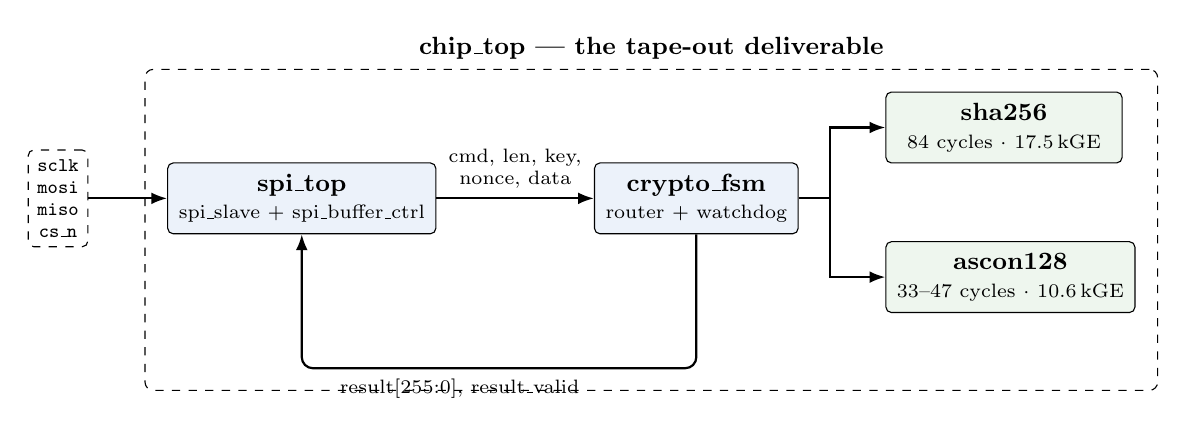
\begin{tikzpicture}[
  node distance=8mm,
  blk/.style={draw,rounded corners=2pt,minimum height=9mm,align=center,
              font=\small,fill=boxfill,inner sep=4pt},
  core/.style={blk,fill=boxfillthree},
  pad/.style={draw,dashed,rounded corners=2pt,minimum height=8mm,align=center,
              font=\scriptsize\ttfamily,fill=white},
  ar/.style={-{Latex[length=2mm]},thick}
]
\node[pad] (pads) {sclk\\mosi\\miso\\cs\_n};
\node[blk,right=10mm of pads,minimum width=26mm] (spi) {\textbf{spi\_top}\\[-1pt]
  \scriptsize spi\_slave + spi\_buffer\_ctrl};
\node[blk,right=20mm of spi,minimum width=24mm] (fsm) {\textbf{crypto\_fsm}\\[-1pt]
  \scriptsize router + watchdog};
\node[core,right=11mm of fsm,yshift=9mm,minimum width=30mm] (sha) {\textbf{sha256}\\[-1pt]
  \scriptsize 84 cycles $\cdot$ 17.5\,kGE};
\node[core,right=11mm of fsm,yshift=-10mm,minimum width=30mm] (asc) {\textbf{ascon128}\\[-1pt]
  \scriptsize 33--47 cycles $\cdot$ 10.6\,kGE};

\draw[ar] (pads) -- (spi);
\draw[ar] (spi) -- node[above,font=\scriptsize,align=center]{cmd, len, key,\\nonce, data} (fsm);
\draw[ar] (fsm.east) -- ++(4mm,0) |- (sha.west);
\draw[ar] (fsm.east) -- ++(4mm,0) |- (asc.west);
\coordinate (ret) at ([yshift=-17mm]fsm.south);
\draw[ar,rounded corners] (fsm.south) -- (ret)
      -| node[pos=0.30,below,font=\scriptsize]{result[255:0], result\_valid} (spi.south);

\begin{scope}[on background layer]
\node[draw,dashed,rounded corners=3pt,inner sep=8pt,
      fit=(spi)(fsm)(sha)(asc)(ret),
      label={[font=\small\bfseries]above:chip\_top --- the tape-out deliverable}] (box) {};
\end{scope}
\end{tikzpicture}
\caption{\texttt{chip\_top}. Everything inside the dashed box was the ASIC
deliverable, and is instantiated on the FPGA with no changes. Gate counts are
from Genus.}
\end{figure}

The intended flow, per the project specification: the host sends the firmware
bytes over SPI with \texttt{CMD = SHA-256}; \texttt{crypto\_fsm} routes the
request to the on-chip core, waits, and returns the digest; the host compares
against a known-good reference and decides whether to allow boot. Note that
\textbf{the boot decision is not made on-chip} --- the chip reports, the host
decides. That is a design limitation worth stating plainly, because a root of
trust that only advises is a weaker guarantee than one that gates.

% =============================================================================
\section{Why the ASIC path did not close}\label{sec:asic}
% =============================================================================

\subsection{The estimate, and the measurement}

The project specification carried a rough pre-synthesis gate estimate. Genus
was then run against the real ETRI library across a frequency sweep. The two
do not agree.

\begin{table}[h]
\centering\small
\begin{tabular}{@{}lrrr@{}}
\toprule
\textbf{Block} & \textbf{Spec estimate} & \textbf{Genus actual} & \textbf{Error} \\
\midrule
SHA-256 core & 10\,000--15\,000\,GE & 17\,455\,GE & 1.2--1.7$\times$ \\
Ascon-128 core & 3\,000--5\,000\,GE & 10\,627\,GE & \textbf{2.1--3.5$\times$} \\
SPI + buffer + router & 1\,000--2\,000\,GE & 11\,252\,GE & \textbf{5.6--11$\times$} \\
Security control FSM & $\sim$350\,GE & (folded into router) & --- \\
\midrule
\textbf{Total} & \textbf{14\,000--22\,000\,GE} & \textbf{39\,333\,GE} &
\textbf{1.8--2.8$\times$} \\
\bottomrule
\end{tabular}
\caption{Pre-synthesis estimate against measured synthesis, at 35\,MHz.
Gate equivalents use the library's own \texttt{NAND2X1} at
216.0\,\textmu m$^2$. The estimate was not absurd --- it was simply never
validated, and the interface logic was underestimated by nearly an order of
magnitude.}
\label{tab:estimate}
\end{table}

The single largest error is not in the cryptography. It is in the plumbing.
\texttt{spi\_buffer\_ctrl} was estimated at a fraction of 1\,000--2\,000\,GE
and came back at \textbf{8\,100\,GE} --- 79\% the size of the entire Ascon
core, for what is conceptually a byte shift register. The reason is visible in
the port list: it holds a 128-bit key, a 128-bit nonce, 256 bits of data and a
256-bit result \emph{simultaneously}, all in flip-flops, all at once.

\subsection{Area against the die budget}

\begin{table}[h]
\centering\small
\begin{tabular}{@{}lrrrrr@{}}
\toprule
\textbf{Block} & \textbf{Cells} & \textbf{Area (\textmu m$^2$)} &
\textbf{mm$^2$} & \textbf{GE} & \textbf{vs 1\,mm$^2$} \\
\midrule
\texttt{sha256}          & 8\,658 & 3\,770\,298 & 3.770 & 17\,455 & \textbf{3.77$\times$} \\
\texttt{ascon128}        & 6\,227 & 2\,295\,423 & 2.295 & 10\,627 & \textbf{2.30$\times$} \\
\texttt{spi\_buffer\_ctrl} & 2\,821 & 1\,749\,609 & 1.750 & 8\,100 & \textbf{1.75$\times$} \\
\texttt{crypto\_fsm} glue & 1\,066 &   608\,000 & 0.608 & 2\,815 & 0.61$\times$ \\
\texttt{spi\_slave}      &    112 &    72\,729 & 0.073 &    337 & 0.07$\times$ \\
\midrule
\textbf{\texttt{chip\_top}} & \textbf{18\,845} & \textbf{8\,496\,018} &
\textbf{8.496} & \textbf{39\,333} & \textbf{8.50$\times$} \\
\bottomrule
\end{tabular}
\caption{Genus \texttt{report\_area}, \texttt{chip\_top} at 35\,MHz, typical
corner. Note the \texttt{Net-Area} column in the raw report is zero and the
wireload model is \texttt{<none>} --- this is \emph{cell area only}. A real
placed and routed die would be larger still, before adding the pad ring.}
\label{tab:area}
\end{table}

\keyfinding{Only \texttt{spi\_slave}, at 0.073\,mm$^2$, would have fit in the
die budget. \textbf{Every other block in the design individually exceeds the
entire 1\,mm$^2$ slot} --- the SHA-256 core by nearly 4$\times$ on its own.}

\begin{figure}[h]
\centering
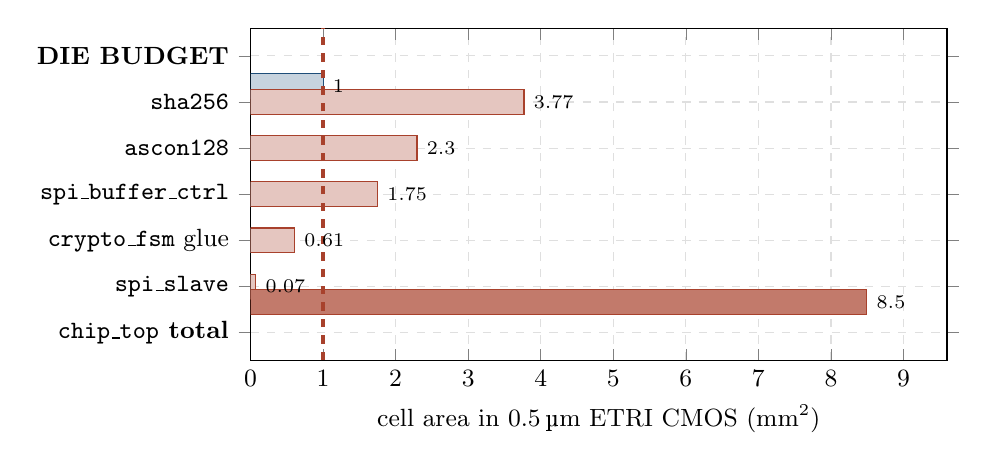
\begin{tikzpicture}
\begin{axis}[
  width=0.86\textwidth, height=5.8cm,
  xbar, xmin=0, xmax=9.6,
  bar width=9pt,
  xlabel={\small cell area in 0.5\,\textmu m ETRI CMOS (mm$^2$)},
  ymin=0.4, ymax=7.6,
  ytick={1,2,3,4,5,6,7},
  yticklabels={{\textbf{\texttt{chip\_top} total}},{\texttt{spi\_slave}},%
    {\texttt{crypto\_fsm} glue},{\texttt{spi\_buffer\_ctrl}},%
    {\texttt{ascon128}},{\texttt{sha256}},{\textbf{DIE BUDGET}}},
  nodes near coords={\pgfmathprintnumber[fixed,precision=2]{\pgfplotspointmeta}},
  nodes near coords style={font=\scriptsize},
  nodes near coords align={horizontal},
  tick label style={font=\small}, label style={font=\small},
  grid=major, grid style={dashed,gray!25},
]
\addplot[fill=signal!25,draw=signal] coordinates {(1.0,7)};
\addplot[fill=accent!30,draw=accent] coordinates {
  (3.770,6) (2.295,5) (1.750,4) (0.608,3) (0.073,2)};
\addplot[fill=accent!70,draw=accent] coordinates {(8.496,1)};
\draw[accent,very thick,dashed] (axis cs:1.0,0.4) -- (axis cs:1.0,7.6);
\end{axis}
\end{tikzpicture}
\caption{Measured area against the 1\,mm$^2$ MPW slot (dashed line). Everything
except \texttt{spi\_slave} is over budget on its own.}
\end{figure}

\subsection{Where the area went}

\begin{table}[h]
\centering\small
\begin{tabular}{@{}lrrr@{}}
\toprule
\textbf{Cell type} & \textbf{Instances} & \textbf{Area (\textmu m$^2$)} & \textbf{Share} \\
\midrule
Sequential (\texttt{DFFSR}) & 2\,985 & 4\,728\,240 & \textbf{55.7\%} \\
Logic & 12\,180 & 3\,205\,431 & 37.8\% \\
Inverters & 3\,636 & 533\,880 & 6.3\% \\
Buffers & 83 & 22\,752 & 0.3\% \\
\midrule
Total & 18\,884 & 8\,490\,303 & 100\% \\
\bottomrule
\end{tabular}
\caption{\texttt{report\_gates} at 50\,MHz. A single \texttt{DFFSR} costs
1\,584\,\textmu m$^2$, or 7.33\,GE. The design is a register file with some
arithmetic attached.}
\end{table}

Flip-flops are the whole story. The architectural state is unavoidable ---
SHA-256 needs 8 working variables, 8 hash registers and a 16-word message
schedule window (1\,024\,b total), Ascon needs a 320-bit permutation state ---
but the \emph{interface} state was a choice. The 256-bit parallel input ports
and the simultaneous key/nonce/data/result buffering exist only because the
protocol was designed to hand each core a whole message at once.

\subsection{Frequency, area and power}

\begin{figure}[h]
\centering
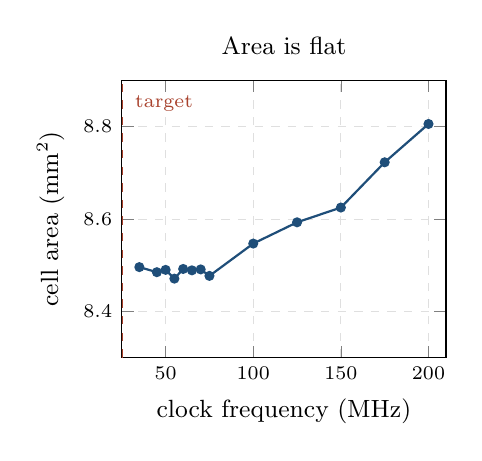
\begin{tikzpicture}
\begin{axis}[
  width=0.47\textwidth, height=5.1cm,
  xlabel={\small clock frequency (MHz)}, ylabel={\small cell area (mm$^2$)},
  xmin=25, xmax=210, ymin=8.3, ymax=8.9,
  tick label style={font=\scriptsize}, label style={font=\small},
  grid=major, grid style={dashed,gray!25},
  title={\small Area is flat}, title style={font=\small},
]
\addplot[signal,mark=*,mark size=1.4pt,thick] coordinates {
 (35,8.496)(45,8.485)(50,8.490)(55,8.471)(60,8.492)(65,8.489)(70,8.491)
 (75,8.477)(100,8.547)(125,8.593)(150,8.625)(175,8.723)(200,8.806)};
\addplot[accent,dashed,thick,forget plot] coordinates {(25,8.3)(25,8.9)};
\node[font=\scriptsize,accent,anchor=west] at (axis cs:27,8.85) {target};
\end{axis}
\end{tikzpicture}\hfill
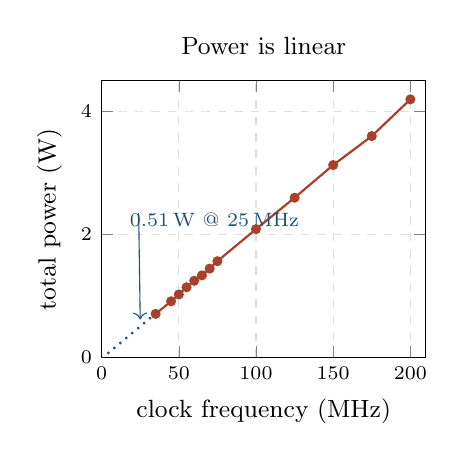
\begin{tikzpicture}
\begin{axis}[
  width=0.47\textwidth, height=5.1cm,
  xlabel={\small clock frequency (MHz)}, ylabel={\small total power (W)},
  xmin=0, xmax=210, ymin=0, ymax=4.5,
  tick label style={font=\scriptsize}, label style={font=\small},
  grid=major, grid style={dashed,gray!25},
  title={\small Power is linear}, title style={font=\small},
]
\addplot[accent,mark=*,mark size=1.4pt,thick] coordinates {
 (35,0.710)(45,0.915)(50,1.026)(55,1.142)(60,1.248)(65,1.336)(70,1.446)
 (75,1.566)(100,2.087)(125,2.597)(150,3.128)(175,3.598)(200,4.195)};
\addplot[signal,dotted,thick,forget plot] coordinates {(0,-0.016)(35,0.716)};
\node[font=\scriptsize,signal,anchor=north west] at (axis cs:12,2.5)
  {0.51\,W @ 25\,MHz};
\draw[signal,thin,->] (axis cs:24,2.35) -- (axis cs:25,0.62);
\end{axis}
\end{tikzpicture}
\caption{Genus PPA sweep, 13 frequency points. Area is essentially constant
from 35 to 75\,MHz and grows only 3.6\% out to 200\,MHz --- confirming the
design is state-bound, not timing-bound. Power fits
$P = 20.9\,\mathrm{mW/MHz} \times f - 16\,\mathrm{mW}$ with $R^2 = 0.9998$,
extrapolating to \textbf{0.51\,W at the 25\,MHz target}.}
\end{figure}

\begin{table}[h]
\centering\small
\setlength{\tabcolsep}{5pt}
\begin{tabular}{@{}rrrrrl@{}}
\toprule
\textbf{Freq (MHz)} & \textbf{Cells} & \textbf{Area (mm$^2$)} &
\textbf{Slack (ps)} & \textbf{Power (W)} & \textbf{Status} \\
\midrule
 35 & 18\,845 & 8.496 & +12\,344 & 0.710 & met \\
 45 & 18\,715 & 8.485 & +5\,721 & 0.915 & met \\
 50 & 18\,884 & 8.490 & +3\,838 & 1.026 & met \\
 55 & 18\,763 & 8.471 & +2\,336 & 1.142 & met \\
 60 & 18\,856 & 8.492 & +820 & 1.248 & met \\
 65 & 18\,948 & 8.489 & +283 & 1.336 & met \\
 70 & 18\,928 & 8.491 & +26 & 1.446 & met \\
 75 & 18\,901 & 8.477 & +2 & 1.566 & met \\
100 & 19\,107 & 8.547 & +103 & 2.087 & met \\
125 & 19\,207 & 8.593 & +6 & 2.597 & met \\
150 & 19\,220 & 8.625 & 0 & 3.128 & met (marginal) \\
175 & 19\,560 & 8.723 & $-$157 & 3.598 & \textbf{violated} \\
200 & 20\,040 & 8.806 & $-$698 & 4.195 & \textbf{violated} \\
\bottomrule
\end{tabular}
\caption{The full sweep. \textbf{$F_{\max}$ in 0.5\,\textmu m is 150\,MHz} ---
six times the 25\,MHz target. The critical path is in \texttt{u\_sha256} at
\emph{every} frequency point, running from \texttt{round\_reg} through the
$\Sigma$/CSA network into \texttt{e\_reg}.}
\label{tab:sweep}
\end{table}

Two things follow from this table.

\textbf{Timing was never the constraint.} The design has 6$\times$ headroom at
the target frequency. All of the effort that would normally go into closing
timing was available to spend on area, and none of it would have been enough:
the gap is 8.5$\times$, not 10\%.

\textbf{Power is a second, independent problem.} 0.51\,W at 25\,MHz is a lot
for a part described as a lightweight root of trust. The cause is the library:
\texttt{khu\_etri05\_stdcells} is characterised at a \textbf{5\,V} nominal
supply, and dynamic power scales with $V^2$. A 1\,mm$^2$ die dissipating half a
watt is also a thermal question, not just an energy one. Leakage is negligible
(2.6\,\textmu W), as expected at this node.

\subsection{On my own earlier estimate}

Before the Genus reports were located, this report carried a bottom-up
reconstruction from the FPGA netlist. It is worth recording how it did, because
the failure mode is instructive.

\begin{table}[h]
\centering\small
\begin{tabular}{@{}lrrl@{}}
\toprule
& \textbf{Reconstruction} & \textbf{Genus actual} & \\
\midrule
Flip-flops & 3\,032 (FPGA) & 2\,985 (\texttt{DFFSR}) & within 1.6\% \\
Gate count & $\sim$33\,kGE & 39\,333\,GE & 16\% low \\
\textmu m$^2$ per GE & 80--90 assumed & \textbf{216.0 measured} & \textbf{2.5$\times$ low} \\
Total area & $\sim$4.4\,mm$^2$ & \textbf{8.496\,mm$^2$} & 1.9$\times$ low \\
\bottomrule
\end{tabular}
\caption{The logical estimate was close. The physical one was not.}
\end{table}

The gate count was recoverable from the FPGA netlist to within 16\%. The area
was not, because I assumed a denser 0.5\,\textmu m library than this one
actually is. \texttt{khu\_etri05\_stdcells} is a 2-poly 3-metal 5\,V analog
CMOS process --- 216\,\textmu m$^2$ per NAND2 against the 80--90 typical of a
digital-optimised 0.5\,\textmu m library. \textbf{The conclusion was right and
the margin was understated by half.} Never scale area across processes without
the actual library.

\subsection{What should have happened}

The project plan had six steps: architectural specs, verification, RTL design,
synthesis, place and route, sign-off. Synthesis was step 4. The area problem
was therefore discovered \emph{after} the RTL was written and verified, which
is the most expensive place to find it.

Three cheap checks, any one of which would have caught it before step 3:

\begin{enumerate}[nosep,leftmargin=1.6em]
\item \textbf{Count the architectural state and multiply.} 1\,024\,b (SHA)
      $+$ 320\,b (Ascon) $+$ 768\,b (SPI buffers) $\approx$ 2\,100 flip-flops
      on paper. At the library's measured 1\,584\,\textmu m$^2$ per
      \texttt{DFFSR} that is 3.3\,mm$^2$ of \emph{registers alone} --- already
      3$\times$ the die. This is arithmetic, not synthesis.
\item \textbf{Synthesise the two cores early}, against the real library, on
      day one of RTL. Genus takes minutes on a design this size.
\item \textbf{Sanity-check the estimate against published work.} Iterative
      SHA-256 is widely reported at 15--22\,kGE; the spec assumed
      10--15\,kGE. Ascon-128 at one round per cycle is published at
      7.9--9.4\,kGE \cite{ascontugraz,springer}; the spec assumed 3--5\,kGE.
      Both estimates were below every published figure.
\end{enumerate}

There is a design answer as well as a planning one. A 1\,mm$^2$ 0.5\,\textmu m
die can hold Ascon-128 --- but only if the wide parallel ports are replaced
with a byte-serial interface and SHA-256 is dropped. Removing SHA-256
(3.77\,mm$^2$) and the buffer controller's parallel storage (1.75\,mm$^2$)
takes 5.5 of the 8.5\,mm$^2$ out at a stroke. That is a different chip, and it
is the chip that would have taped out.

% =============================================================================
\section{The pivot to FPGA}\label{sec:pivot}
% =============================================================================

Once the die was clearly out of reach, the work was redirected to producing a
verified core plus a hardware platform that proves it. The RTL defects are real
regardless of target; an FPGA gives a measurable baseline the ASIC path was
never going to produce; and timing closure at 100\,MHz is strictly harder than
at the 25\,MHz ASIC target.

The board was a ZCU106 (XCZU7EV-FFVC1156-2-E), Vivado 2025.1.

\subsection{Two decisions worth defending}

\textbf{A custom AXI4-Lite peripheral, not AXI Quad SPI.} The obvious route is
to drop in Xilinx's AXI Quad SPI IP as the master. I wrote a small custom
peripheral instead, for one reason: the whole PS-to-PL path can then be
simulated end to end against a real AXI4-Lite bus-functional model, and IP GUI
settings cannot. AXI Quad SPI has a build-time frequency ratio, a slave-select
register, FIFO behaviour and an \texttt{XSpi} driver with real subtleties
around manual slave select --- every one of those is a place to lose a day
during bring-up. The custom peripheral also has a \emph{runtime}-settable clock
divider, which is what made the SCLK margin sweep possible on hardware. The
cost is about 300 lines of Verilog that we own.

\textbf{One clock domain.} The AXI interface, the SPI master and
\texttt{chip\_top} all run on \texttt{pl\_clk0}. No clock domain crossing
anywhere, the SPI path is an ordinary register-to-register path that static
timing analysis fully covers, and there are no I/O timing constraints to get
wrong. Behaviour is identical to a 25\,MHz clock because the design is fully
synchronous --- what matters is the SCLK-to-clock \emph{ratio}, not the
absolute frequency.

\begin{figure}[h]
\centering
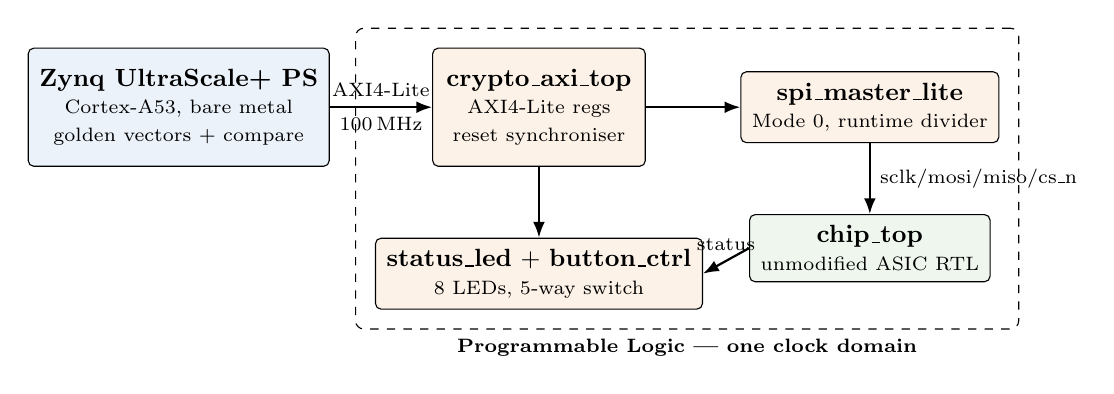
\begin{tikzpicture}[
  node distance=7mm,
  blk/.style={draw,rounded corners=2pt,minimum height=8mm,align=center,
              font=\small,fill=boxfill,inner sep=4pt},
  fpgablk/.style={blk,fill=boxfilltwo},
  asicblk/.style={blk,fill=boxfillthree},
  ar/.style={-{Latex[length=2mm]},thick}
]
\node[blk,minimum width=30mm,minimum height=15mm] (ps)
  {\textbf{Zynq UltraScale+ PS}\\[-1pt]\scriptsize Cortex-A53, bare metal\\[-1pt]
   \scriptsize golden vectors + compare};
\node[fpgablk,right=13mm of ps,minimum width=27mm,minimum height=15mm] (axi)
  {\textbf{crypto\_axi\_top}\\[-1pt]\scriptsize AXI4-Lite regs\\[-1pt]
   \scriptsize reset synchroniser};
\node[fpgablk,right=12mm of axi,minimum width=25mm] (mst)
  {\textbf{spi\_master\_lite}\\[-1pt]\scriptsize Mode 0, runtime divider};
\node[asicblk,below=9mm of mst,minimum width=25mm] (chip)
  {\textbf{chip\_top}\\[-1pt]\scriptsize unmodified ASIC RTL};
\node[fpgablk,below=9mm of axi,minimum width=27mm] (io)
  {\textbf{status\_led} + \textbf{button\_ctrl}\\[-1pt]\scriptsize 8 LEDs, 5-way switch};

\draw[ar] (ps) -- node[above,font=\scriptsize]{AXI4-Lite} node[below,font=\scriptsize]{100\,MHz} (axi);
\draw[ar] (axi) -- (mst);
\draw[ar] (mst) -- node[right,font=\scriptsize]{sclk/mosi/miso/cs\_n} (chip);
\draw[ar] (axi) -- (io);
\draw[ar] (chip.west) -- node[above,font=\scriptsize]{status} (io.east);

\begin{scope}[on background layer]
\node[draw,dashed,rounded corners=3pt,inner sep=7pt,
      fit=(axi)(mst)(chip)(io),
      label={[font=\scriptsize\bfseries]below:Programmable Logic --- one clock domain}] {};
\end{scope}
\end{tikzpicture}
\caption{The ZCU106 validation platform. Orange blocks are FPGA-only
scaffolding and are not intended to tape out; green is the ASIC deliverable,
instantiated with no changes.}
\end{figure}

% =============================================================================
\section{What was wrong with the RTL}\label{sec:rtl}
% =============================================================================

Six defects. Five were confirmed by running the original code in simulation,
not by reading it.

\subsection{Ascon-128 produced the wrong authentication tag}

\textbf{Critical.} Ascon requires the plaintext to be padded with \texttt{0x80}
followed by zeros up to a multiple of the 8-byte rate, and critically \emph{a
full padding block is appended even when the length is already a multiple of
8}. The original core skipped the padding block entirely.

The ciphertext still came out correct, because the padding block contributes no
ciphertext bytes. But the padding block is absorbed into the state before
finalisation, so the tag was wrong for every single input:

{\small
\begin{verbatim}
pt_len=0   tag got 2cd6a332f04aaf580df298a559aa76a9
           tag exp e355159f292911f794cb1432a0103a8a   <- NIST LWC KAT

pt_len=16  ct  got bc820dbdf7a4631c5b29884ad69175c3   <- ciphertext correct
           tag got f949e005f483688490270dd7033dfba5
           tag exp f58e28436dd71556d58dfa56ac890beb   <- tag wrong
\end{verbatim}}

A wrong tag is the worst kind of failure here: encryption looks like it works,
and the fault only surfaces when someone tries to decrypt or authenticate. For
a part whose stated job is authenticating device identity and transmitted data
on naval equipment, this is the defect that matters most.

Fixed by implementing the padding inside the core, including the ciphertext
truncation mask so pad bytes never leak into the output. It now passes all 37
vectors covering every plaintext length 0 to 32, plus associated-data cases.

\subsection{Result transmission never terminated}

\texttt{byte\_idx} in \texttt{spi\_buffer\_ctrl} was \texttt{reg [4:0]}, so it
counted 0 to 31. The transmit loop exited on
\texttt{byte\_idx >= result\_len\_latch} with \texttt{result\_len\_latch}
always 32. A 5-bit counter can never reach 32, so the comparison was never
true. The FSM streamed 32 correct bytes, then wrapped to 0 and kept streaming
zeros forever, never returning to idle. The observable symptom: the first
command works, and every command after it is silently ignored.

\subsection{MISO was one bit early from the second byte onward}

The controller asserts \texttt{tx\_load} a few system clocks after a byte
completes, which lands \emph{before} the SCLK falling edge that ends that bit
period. The original code applied the load straight to the shift register, so
that falling edge shifted the freshly loaded byte one more time:

{\small
\begin{verbatim}
got 63 1b 9b 53 cd 89 ...
exp 63 0d cd 29 66 c4 ...
     ^  ^^ every byte after the first is shifted left by one bit
\end{verbatim}}

This is the kind of bug that passes a core-level testbench and only appears
once you drive real SPI traffic. Fixed by staging the incoming byte in
\texttt{tx\_hold}/\texttt{tx\_pending} and swapping it into the shifter
\emph{on} the falling edge, which is the actual byte boundary.

\subsection{The other three}

\begin{itemize}[nosep,leftmargin=1.4em]
\item \textbf{Message alignment mismatch.} \texttt{spi\_buffer\_ctrl}
      accumulated bytes by shifting into the LSB end, leaving the message
      right-aligned; both cores expect it left-aligned. The two only agree when
      \texttt{DATA\_LEN} is exactly 32, so any shorter message hashed the wrong
      block --- which for a firmware-integrity part means the wrong digest.
\item \textbf{Zero-length input hung the receive loop.} \texttt{S\_RX\_DATA}
      exited on \texttt{byte\_idx == data\_len\_out - 1}; with
      \texttt{data\_len\_out} zero that is \texttt{0xFF}, never reached.
\item \textbf{Unrecognised commands still ran SHA-256.} A request with neither
      command bit set fell into the SHA branch and returned a
      plausible-looking wrong answer. Commands and lengths are now validated
      and raise \texttt{err}.
\end{itemize}

\subsection{Also corrected}

\begin{itemize}[nosep,leftmargin=1.4em]
\item \textbf{The documented SCLK limit was wrong, and the spec's SPI clock is
      not achievable.} The header claimed $f_{\mathrm{clk}}/2$. Sweeping the
      rate in simulation, the design passes at $f_{\mathrm{clk}}/6$ and fails
      at $f_{\mathrm{clk}}/4$; the documented limit is now
      $f_{\mathrm{clk}}/8$. \textbf{The project specification calls for a
      5\,MHz SPI clock at a 25\,MHz system clock} --- that is
      $f_{\mathrm{clk}}/5$, above the safe limit and inside the measured
      failure band. Either the system clock has to rise or the SPI clock has to
      drop. This was not previously flagged anywhere.
\item \textbf{Frame abort recovery.} A frame ending early used to leave the FSM
      stuck until reset. Receive states now abort cleanly back to idle, which
      matters during bring-up: one glitch no longer means a board reset.
\item \textbf{Watchdog.} If a core never asserted \texttt{done} the chip locked
      up forever. \texttt{crypto\_fsm} now bounds the wait and returns an
      error result.
\item \textbf{Reset domain crossing.} \texttt{rst\_n} was used as an
      asynchronous reset in some blocks and a synchronous reset in others, so
      different parts of the design could leave reset on different clock edges
      --- intermittent start-up failures that are very hard to reproduce. The
      FPGA wrapper now contains a proper async-assert / sync-release reset
      synchroniser.
\end{itemize}

% =============================================================================
\section{Verification}\label{sec:verif}
% =============================================================================

\begin{table}[h]
\centering\small
\begin{tabular}{@{}llc@{}}
\toprule
\textbf{Test} & \textbf{What it covers} & \textbf{Result} \\
\midrule
\texttt{button\_unit} & debounce, both-press window, hold, glitch rejection & pass \\
\texttt{sha256\_unit} & 36 vectors, every length 0--32, against Python \texttt{hashlib} & pass \\
\texttt{ascon\_unit}  & 37 vectors, every length 0--32 plus associated-data cases & pass \\
\texttt{chip\_e2e}    & 29 vectors through the real SPI pins, plus rejection and abort & pass \\
\texttt{axi\_stack}   & 17 checks through an AXI4-Lite bus-functional model & pass \\
\texttt{sclk\_margin} & SCLK rate sweep to find the actual failure point & characterised \\
lint & Verilator \texttt{-Wall} on \texttt{chip\_top} and \texttt{crypto\_axi\_top} & clean \\
C build & \texttt{gcc -Wall -Wextra} on the Vitis application & clean \\
\midrule
\textbf{Hardware} & ZCU106, Vitis on \texttt{psu\_cortexa53\_0} & \textbf{all pass} \\
\bottomrule
\end{tabular}
\caption{The full suite, re-run for this report. The Ascon golden reference is
validated against the published NIST LWC known-answer test: key and nonce
\texttt{000102...0F}, empty AD, empty plaintext gives tag
\texttt{E355159F292911F794CB1432A0103A8A}.}
\end{table}

\textbf{The SCLK margin sweep.} $f_{\mathrm{clk}}/16$, $/10$, $/8$ and $/6$
pass; $/4$ and $/2$ fail. Edge detection compares adjacent synchroniser stages,
and the TX byte handover needs three system clocks between a rising edge and
the following falling edge, so the limit is structural rather than arbitrary.

\textbf{On hardware.} The bitstream was programmed onto the ZCU106 and the
bare-metal application launched on \texttt{psu\_cortexa53\_0} from Vitis. The
first thing it does is read the ID register at offset \texttt{0x00}, which
returns \texttt{0x5AA5C0DE}: if that reads back correctly then the bitstream,
clock, reset, address map and AXI path are all working, and any later failure
is a logic problem rather than an infrastructure problem. It then pushes known
vectors through the real SPI pins and compares on the A53. Every vector in the
run passed and all eight LEDs went solid.

The application holds 200 SHA-256 and 200 Ascon-128 known-answer vectors and
draws a random subset per button press, seeded from the CPU cycle counter at
the moment of the press, plus three negative tests (bad command, oversize
length, recovery). So a single run exercises a different sample each time
rather than the same fixed list --- which is the right behaviour for catching
input-dependent faults, but it does mean the pass count printed over UART
depends on the build's \texttt{SHA\_PER\_RUN} / \texttt{ASC\_PER\_RUN}
settings rather than being a fixed figure.

The eight user LEDs are driven as one bar rather than a red/green pair, because
the ZCU106's user LEDs are single-colour. Idle is a slow pulse
(\textasciitilde 0.38\,Hz), running is a fast even blink
(\textasciitilde 6\,Hz), pass is solid on, fail is dark. Anything moving means
``no verdict yet''; anything static is the answer. Idle deliberately pulses
rather than sitting dark --- otherwise a board waiting at the menu, a crashed
application and a bitstream that never programmed would all look identical to a
failing test.

% =============================================================================
\section{Measured FPGA results}\label{sec:results}
% =============================================================================

\subsection{Resource utilisation and timing}

\begin{table}[h]
\centering\small
\begin{tabular}{@{}lrrrrr@{}}
\toprule
\textbf{Module} & \textbf{LUT} & \textbf{FF} & \textbf{CARRY8} &
\textbf{WNS (ns)} & \textbf{$F_{\max}$ (MHz)} \\
\midrule
\texttt{sha256}      & 1\,188 & 1\,302 & 52 & 5.832 & 240 \\
\texttt{ascon128}    & 1\,341 &    728 &  0 & 7.219 & 360 \\
\texttt{crypto\_fsm} & 2\,603 & 2\,179 & 52 & 6.011 & 251 \\
\texttt{spi\_top}    &    608 &    862 &  0 & 7.914 & 479 \\
\midrule
\texttt{chip\_top} (ASIC deliverable) & 3\,232 & 3\,032 & 52 & 5.740 & 235 \\
\midrule
Full system, placed \& routed & 3\,923 & 3\,885 & 71 & 5.868 & \textbf{242} \\
\bottomrule
\end{tabular}
\caption{XCZU7EV-FFVC1156-2-E, Vivado 2025.1. Rows 1--5 are out-of-context
synthesis, place and route with a 10\,ns constraint. The last row is the
complete block design including the AXI SmartConnect, LEDs and buttons.
$F_{\max}$ is $1/(T - \mathrm{WNS})$, which is optimistic: the tools stop
optimising once the constraint is met.}
\label{tab:util}
\end{table}

Zero BRAM, zero URAM, zero DSP. 781 CLBs, 185 unique control sets. The FPGA's
3\,032 flip-flops for \texttt{chip\_top} agree with Genus's 2\,985 to within
1.6\%, which is a useful cross-check that the two flows are building the same
design.

\subsection{Power}

\begin{table}[h]
\centering\small
\begin{tabular}{@{}lrl@{}}
\toprule
\textbf{Component} & \textbf{Power} & \textbf{Note} \\
\midrule
\texttt{crypto\_axi\_top} (all PL logic) & \textbf{31\,mW} & the number that means anything \\
AXI SmartConnect & 5\,mW & interconnect overhead \\
PS8 (Cortex-A53 subsystem) & 2\,656\,mW & fixed Vivado estimate for the MPSoC \\
Device static & 692\,mW & 593\,mW PL, 98\,mW PS \\
\midrule
Total on-chip & 3\,386\,mW & \\
\bottomrule
\end{tabular}
\caption{\texttt{report\_power} on the routed design, 100\,MHz, default
switching activity. Confidence level: low --- no SAIF was back-annotated, so
treat 31\,mW as an upper-bound estimate rather than a measurement. The headline
3.4\,W is almost entirely the hard processor system and the static leakage of a
large FPGA; neither has anything to do with the crypto design.}
\end{table}

The FPGA's 31\,mW and the ASIC's 0.51\,W are not directly comparable --- 16\,nm
FinFET at 0.85\,V against 0.5\,\textmu m at 5\,V is a 30-year gap --- but the
contrast is worth stating, because it is the strongest practical argument for
not reviving the 0.5\,\textmu m target.

\subsection{Latency, measured in simulation}

\begin{table}[h]
\centering\small
\begin{tabular}{@{}llrrr@{}}
\toprule
\textbf{Core} & \textbf{Case} & \textbf{Cycles} &
\textbf{@ 25\,MHz} & \textbf{@ 100\,MHz} \\
\midrule
SHA-256 & any length 0--32\,B & 84 & 3.36\,\textmu s & 0.84\,\textmu s \\
Ascon-128 & \texttt{pt\_len}=0 & 33 & 1.32\,\textmu s & 0.33\,\textmu s \\
Ascon-128 & \texttt{pt\_len}=8 & 40 & 1.60\,\textmu s & 0.40\,\textmu s \\
Ascon-128 & \texttt{pt\_len}=16 & 47 & 1.88\,\textmu s & 0.47\,\textmu s \\
Ascon-128 & \texttt{pt\_len}=16, \texttt{ad\_len}=16 & 71 & 2.84\,\textmu s & 0.71\,\textmu s \\
\bottomrule
\end{tabular}
\caption{Cycle counts measured with a dedicated testbench, counting from the
\texttt{start} pulse to \texttt{done}. Ascon costs a flat 7 cycles per
additional 64-bit rate block (1 absorb $+$ 6 permutation rounds). SHA-256
breaks down as 1 (pad) $+$ 16 (schedule load) $+$ 64 (compress) $+$ 2 (output).}
\end{table}

\subsection{The system is I/O bound, not compute bound}
\label{sec:iobound}

This is the most important measurement in the report and it was not in the
original specification.

At the ASIC target --- 25\,MHz system clock, SCLK capped at
$f_{\mathrm{clk}}/8 = 3.125$\,MHz --- one SPI byte takes 2.56\,\textmu s. A
32-byte SHA-256 request needs a 34-byte command frame and a 32-byte readback
frame.

\begin{figure}[h]
\centering
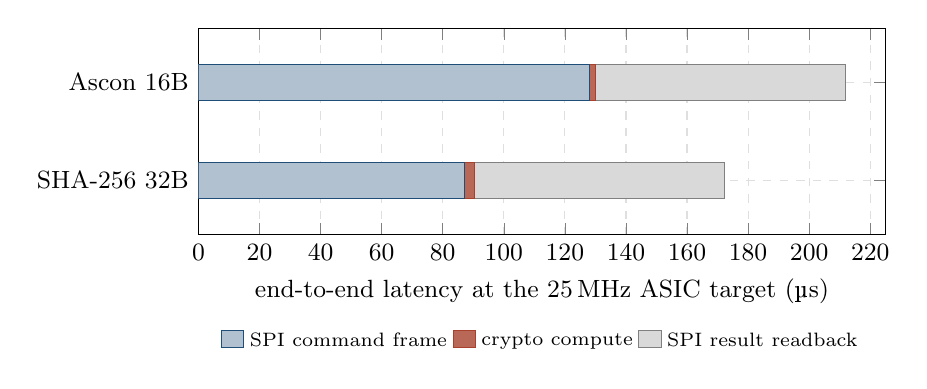
\begin{tikzpicture}
\begin{axis}[
  width=0.85\textwidth, height=4.2cm,
  xbar stacked, xmin=0, xmax=225,
  bar width=13pt,
  xlabel={\small end-to-end latency at the 25\,MHz ASIC target (\textmu s)},
  symbolic y coords={Ascon 16B,SHA-256 32B},
  ytick=data, y dir=reverse,
  tick label style={font=\small}, label style={font=\small},
  legend style={font=\scriptsize,at={(0.5,-0.42)},anchor=north,legend columns=3,draw=none},
  grid=major, grid style={dashed,gray!25},
  enlarge y limits=0.55,
]
\addplot[fill=signal!35,draw=signal] coordinates {(87.04,SHA-256 32B) (128.0,Ascon 16B)};
\addplot[fill=accent!80,draw=accent] coordinates {(3.36,SHA-256 32B) (1.88,Ascon 16B)};
\addplot[fill=gray!30,draw=gray] coordinates {(81.92,SHA-256 32B) (81.92,Ascon 16B)};
\legend{SPI command frame, crypto compute, SPI result readback}
\end{axis}
\end{tikzpicture}
\caption{Where the time actually goes. The red slice is the entire reason the
chip exists. It is 1.9\% of a SHA-256 transaction and 0.9\% of an Ascon
transaction.}
\end{figure}

\begin{table}[h]
\centering\small
\begin{tabular}{@{}lrrrr@{}}
\toprule
\textbf{Operation} & \textbf{Total} & \textbf{Compute share} &
\textbf{Effective} & \textbf{Core capability} \\
\midrule
SHA-256, 32\,B & 172.3\,\textmu s & 1.9\% & 1.49\,Mbps & 152\,Mbps \\
Ascon-128, 16\,B & 211.8\,\textmu s & 0.9\% & 0.60\,Mbps & 229\,Mbps \\
\bottomrule
\end{tabular}
\caption{At 25\,MHz with SCLK at $f_{\mathrm{clk}}/8$. ``Core capability'' is
the sustained rate the core could deliver if data arrived instantly.}
\end{table}

\keyfinding{The cores are starved by factors of roughly 100 and 380. For a
firmware-integrity part this compounds: hashing a 1\,MB firmware image 32 bytes
at a time, at 172\,\textmu s per transaction, takes about \textbf{5.6 seconds}
--- and the SHA-256 core is idle for 98\% of it.}

% =============================================================================
\section{Comparison with published implementations}\label{sec:compare}
% =============================================================================

\subsection{SHA-256}

\begin{table}[h]
\centering\small
\setlength{\tabcolsep}{4pt}
\begin{tabular}{@{}llrrrrr@{}}
\toprule
\textbf{Work} & \textbf{Device} & \textbf{LUT} & \textbf{FF} &
\textbf{Freq} & \textbf{Cyc/blk} & \textbf{Thr.} \\
\midrule
\textbf{This work} & XCZU7EV & \textbf{1\,188} & \textbf{1\,302} &
  240\,MHz & \textbf{84} & 1.46\,Gbps \\
\textbf{This work} & 0.5\,\textmu m ETRI & \multicolumn{2}{c}{17\,455\,GE} &
  25\,MHz & 84 & 0.15\,Gbps \\
\midrule
secworks/sha256 \cite{secworks} & Artix-7 xc7a200t & 2\,471 & 1\,930 &
  108\,MHz & 66 & 0.84\,Gbps \\
secworks/sha256 \cite{secworks} & Spartan-6 & 2\,012 & 1\,929 &
  70\,MHz & 66 & 0.54\,Gbps \\
MDPI Sensors 2024, 1 core \cite{mdpi} & Virtex-6 & 6\,730 & 794 &
  12.7\,MHz & 65 & 0.10\,Gbps \\
Ref.~[38] in \cite{mdpi} & Artix-7 & 1\,310 & 881 &
  141.8\,MHz & --- & 1.40\,Gbps \\
Unfolded, in \cite{mdpi} & Arria II GX & 1\,215 & 871 &
  --- & 32 & 2.43\,Gbps \\
\midrule
secworks/sha256 \cite{secworks} & 40\,nm LP ASIC & \multicolumn{2}{c}{14\,200\,\textmu m$^2$} &
  250\,MHz & 66 & 1.94\,Gbps \\
\bottomrule
\end{tabular}
\caption{Throughput is $512 \times f / \text{cycles per block}$. Frequency
comparisons across device families are not meaningful; \textbf{cycles per
block} is the number to read.}
\end{table}

\textbf{Where we stand.} 17.5\,kGE sits inside the published 15--22\,kGE range
for an iterative SHA-256, and 1\,188 LUT / 1\,302 FF is at the small end of the
FPGA field. But this is partly an unfair comparison: our core handles a
\emph{single} 512-bit block with a fixed 256-bit input port and no streaming,
so it does not carry the multi-block control a general-purpose core needs. A
core that cannot hash more than 32 bytes is not really comparable to one that
can hash a file.

\textbf{Where we are behind: 84 cycles per block against a field of 65--66.}
That is 27\% slower for no architectural reason. Our core loads all 16
message-schedule words serially before starting compression, when the standard
approach folds the load into the first 16 compression rounds ---
$W[0..15]$ are consumed one per round anyway. Fixing this brings us to
\textasciitilde 67 cycles and costs no area. Given that the critical path also
lives in this core at every frequency point (Table~\ref{tab:sweep}), it is the
obvious place to spend effort.

\subsection{Ascon-128}

\begin{table}[h]
\centering\small
\setlength{\tabcolsep}{4pt}
\begin{tabular}{@{}llrrrr@{}}
\toprule
\textbf{Work} & \textbf{Platform} & \textbf{Rnd/cyc} & \textbf{LUT} &
\textbf{FF} & \textbf{Area / Thr.} \\
\midrule
\textbf{This work} & XCZU7EV & 1 & \textbf{1\,341} & \textbf{728} &
  3.28\,Gbps @ 360\,MHz \\
\textbf{This work} & 0.5\,\textmu m ETRI & 1 & \multicolumn{2}{c}{\textbf{10\,627\,GE}} &
  0.23\,Gbps @ 25\,MHz \\
\midrule
Malal \cite{asconvhdl} & Artix-7 & 6 & 2\,957 & 595 & 3.54\,Gbps @ 55\,MHz \\
Malal \cite{asconvhdl} & Kintex-7 & 6 & 2\,958 & 595 & 5.93\,Gbps @ 93\,MHz \\
Malal \cite{asconvhdl} & Spartan-7 & 6 & 2\,957 & 595 & 3.44\,Gbps @ 54\,MHz \\
As tabulated in \cite{survey} & Artix-7 & --- & 1\,756 & 912 & 0.38\,Gbps @ 55\,MHz \\
\midrule
Gro\ss{} (CAESAR HW API) \cite{ascontugraz} & ASIC & 1 & \multicolumn{2}{c}{9\,420\,GE} & 4.89\,Gbps \\
Gro\ss{} (CAESAR HW API) \cite{ascontugraz} & ASIC & 2 & \multicolumn{2}{c}{12\,989\,GE} & 8.48\,Gbps \\
Gro\ss{} (CAESAR HW API) \cite{ascontugraz} & ASIC & 6 & \multicolumn{2}{c}{27\,280\,GE} & 12.26\,Gbps \\
Optimised IoT design \cite{springer} & ASIC & 1 & \multicolumn{2}{c}{7\,891\,GE} & --- \\
\bottomrule
\end{tabular}
\caption{Our Ascon core is a 1-round-per-cycle iterative design, so the
1-round ASIC rows are the fair comparison.}
\end{table}

\textbf{Where we stand.} 10\,627\,GE against Gro\ss{}'s 9\,420\,GE for the same
1-round-per-cycle architecture \cite{ascontugraz} and 7\,891\,GE for an
area-optimised design \cite{springer}. We are 13\% larger than the CAESAR-API
reference and 35\% larger than the best published --- respectable, but not
best-in-class, and the gap is almost certainly the 256-bit \texttt{ad} and
\texttt{plaintext} input ports, which hold data the core consumes 64 bits at a
time. On FPGA, 1\,341 LUT is smaller than every design in the table, and it
closes at 360\,MHz, the fastest block in the design by a wide margin.

\textbf{Where we are behind: rounds per cycle.} Every high-performance design
in the literature unrolls. Malal's 6-round unroll \cite{asconvhdl} finishes a
64-bit block in 2 cycles instead of 7, and Gro\ss{}'s ASIC data shows the trade
curve directly: $1 \to 2$ rounds costs 38\% more area for 73\% more throughput.
For a 25\,MHz ASIC with 6$\times$ timing headroom that was the wrong trade ---
but on the FPGA it is a straightforward win.

% =============================================================================
\section{What still needs work}\label{sec:next}
% =============================================================================

Ordered by value per unit of effort.

\textbf{1. Overlap the SHA-256 message schedule with compression.}
84 $\to$ \textasciitilde 67 cycles, a 20\% latency cut, at no area cost. The
16 schedule words are consumed one per round; there is no reason to load them
in a separate 16-cycle phase first. \emph{Effort: half a day. Risk: low --- the
36-vector unit test catches any mistake immediately.}

\textbf{2. Widen the host interface, or the chip is pointless.} The
measurements in Section~\ref{sec:iobound} show the SPI link is 98--99\% of
every transaction. Three options, in increasing order of work:
\begin{itemize}[nosep,leftmargin=1.4em]
\item Raise SCLK. The measured failure point is $f_{\mathrm{clk}}/4$; the
      documented limit is $f_{\mathrm{clk}}/8$. Restructuring the TX byte
      handover so it does not need three system clocks between edges would make
      $f_{\mathrm{clk}}/4$ safe --- a straight 2$\times$, and it would also make
      the specification's 5\,MHz SPI clock legal.
\item Use quad SPI, or a parallel bus. 4$\times$ for the data phases.
\item Overlap. Nothing today lets the host stream the next command while the
      previous result is being read. Double-buffering the result register would
      hide the entire readback frame behind the next command.
\end{itemize}
\emph{Effort: 1--3 days depending on option. Risk: medium --- the SPI timing is
where the original bugs lived, so the margin sweep must be re-run.}

\textbf{3. Remove the 32-byte ceiling.} Both cores are single-block. SHA-256
cannot hash anything longer than 32 bytes, which for a firmware-integrity part
is close to disqualifying --- real firmware images are megabytes. Ascon is
capped at 16 bytes of plaintext by the 256-bit result bus, not by the core.
Multi-block streaming means feeding the core a block at a time and keeping the
chaining value; for SHA-256 this is mostly control logic, and the compression
function does not change. \emph{Effort: 3--5 days. Risk: medium.}

\textbf{4. Move the boot decision on-chip.} Today the chip returns a digest and
the host compares it. That means the comparison --- the actual security
decision --- happens in software the chip is supposed to be protecting.
Storing a reference digest in on-chip OTP and driving a
\texttt{boot\_ok}/\texttt{boot\_error} pin directly would close that gap, and
it is already drawn that way in the project's own architecture diagram.
\emph{Effort: 2--3 days plus an OTP macro. Risk: medium.}

\textbf{5. Expose associated data.} \texttt{ad\_len} is tied to zero in the SPI
protocol. The core implements AD correctly and it is covered by the unit tests,
so this is a protocol change, not a core change. Without it the Ascon interface
is not really AEAD, only AE. \emph{Effort: 1 day. Risk: low.}

\textbf{6. Add Ascon decryption and tag verification.} Encryption only, today.
An AEAD core that cannot verify is half a core, and constant-time tag
comparison in hardware is straightforward. \emph{Effort: 2--3 days.}

\textbf{7. Side-channel resistance --- nothing has been done here.} This is a
key-handling part for defence equipment with an unprotected datapath. The key
sits in a plain register and the permutation is unmasked. Published protected
Ascon designs run around 41\,kGE against 9\,kGE unprotected \cite{survey}, a
4.5$\times$ area penalty, so this is a design-level decision that has to be
made up front, not retrofitted. \emph{Nobody should ship this against a
physical-access threat model as it stands.}

\textbf{8. If the ASIC is revived, re-scope before writing any RTL.}
Table~\ref{tab:area} says what to cut. Dropping SHA-256 removes 3.77\,mm$^2$;
replacing the parallel input ports with a byte-serial interface removes most of
\texttt{spi\_buffer\_ctrl}'s 1.75\,mm$^2$. That takes 8.5\,mm$^2$ down toward
3\,mm$^2$ --- still over a 1\,mm$^2$ slot, so either the die grows or a newer
node is used. At 0.5\,\textmu m and 216\,\textmu m$^2$ per gate, 1\,mm$^2$ buys
about 4\,600 gates. That is the real budget, and it should be the first number
in the next specification.

\textbf{9. Housekeeping.} The Vivado build script
(\texttt{scripts/build\_zcu106.tcl}) has never been executed against a real
Vivado installation --- the manual block-design flow is the reliable path. All
pin assignments come from the ZCU106 Rev1.0 master XDC; a different board
revision needs re-checking, because wrong pins still build and the LEDs simply
never light. Genus was also run without a wireload model
(\texttt{Net-Area = 0}), so the 8.5\,mm$^2$ is a floor, not a final number ---
a physical-aware run with the supplied LEF and QRC tech files would give the
real figure.

% =============================================================================
\section{Reproducing this}\label{sec:repro}
% =============================================================================

All sources are at \url{https://github.com/tk685-cpu/trustcore} (the working
copy on the lab machine is \texttt{\textasciitilde/Desktop/trustcore\_vivado}).
The layout of the repository is:

{\small
\begin{verbatim}
rtl/                  ASIC deliverable -- instantiated unmodified
  chip_top.v          top level, status pins
  spi_top.v spi_slave.v spi_buffer_ctrl.v
  crypto_fsm.v        command validation, watchdog
  sha256.v            iterative, 84 cycles/block
  ascon128.v          spec-compliant padding
rtl_fpga/             FPGA-only scaffolding -- not for tape-out
  crypto_axi_top.v    AXI4-Lite peripheral, reset synchroniser
  spi_master_lite.v   SPI Mode 0 master, runtime divider
  status_led.v button_ctrl.v
synthesis/            Genus flow
  genus.tcl constraints.sdc run_sweep.sh
  reports/            13 frequency points, area/gates/power/timing
  netlist/chip_top_genus.v
lib/                  khu_etri05_stdcells.lib, LEF, GDS2, QRC tech files
constraints/zcu106_crypto.xdc
scripts/run_sim.sh    the whole verification suite
vitis/main.c          bare-metal validation application
sim/                  testbenches + Python golden reference
plot/plot_ppa.py      the PPA sweep charts
\end{verbatim}}

Simulation: \texttt{cd scripts \&\& ./run\_sim.sh}, requires \texttt{iverilog},
\texttt{python3}, optionally \texttt{verilator}. Synthesis:
\texttt{cd synthesis \&\& ./run\_sweep.sh}, requires Genus and the ETRI library.

\begin{center}
\fbox{\parbox{0.93\textwidth}{\small On the lab machine the Xilinx tools put an
old \texttt{libstdc++} on \texttt{LD\_LIBRARY\_PATH}, which breaks
\texttt{iverilog} with \texttt{GLIBCXX\_3.4.32 not found}. Run
\texttt{env -u LD\_LIBRARY\_PATH ./run\_sim.sh} instead.}}
\end{center}

% =============================================================================
\section*{References}
% =============================================================================
\small
\begin{thebibliography}{9}
\bibitem{secworks} J. Str\"ombergson, \emph{secworks/sha256 --- Hardware
implementation of the SHA-256 cryptographic hash function}. FPGA and 40\,nm
ASIC results in the project README.
\url{https://github.com/secworks/sha256}

\bibitem{mdpi} \emph{SHA-256 Hardware Proposal for IoT Devices in the
Blockchain Context}, Sensors 24(12):3908, MDPI, 2024. Comparison table of
SHA-256 FPGA implementations 2002--2021.
\url{https://www.mdpi.com/1424-8220/24/12/3908}

\bibitem{ascontugraz} \emph{Ascon --- Implementations}, Institute of Applied
Information Processing and Communications, TU Graz. CAESAR Hardware API ASIC
results by H.\ Gro\ss{}.
\url{https://ascon.isec.tugraz.at/implementations.html}

\bibitem{asconvhdl} A. Malal, \emph{ascon-vhdl}, and
\emph{High-Performance FPGA Implementations of Lightweight ASCON-128 and
ASCON-128a with Enhanced Throughput-to-Area Efficiency}, IACR ePrint 2025/825.
\url{https://github.com/AhmetMALAL/ascon-vhdl},
\url{https://eprint.iacr.org/2025/825}

\bibitem{survey} J. Kaur, A. Cintas Canto, M. Mozaffari Kermani,
R. Azarderakhsh, \emph{A Comprehensive Survey on the Implementations, Attacks,
and Countermeasures of the Current NIST Lightweight Cryptography Standard},
arXiv:2304.06222, 2023. \url{https://arxiv.org/abs/2304.06222}

\bibitem{springer} \emph{An Optimized Hardware Implementation of ASCON Cipher
for IoT Applications}, Springer, 2024.
\url{https://link.springer.com/chapter/10.1007/978-981-97-3756-7_22}

\bibitem{nist} NIST Lightweight Cryptography project, Ascon known-answer test
vectors. \url{https://csrc.nist.gov/projects/lightweight-cryptography}
\end{thebibliography}

\end{document}
